%%%%%%%%%%%%%%%%%%%%%%%%%%%%%%%%%%%%%%%%%
% Beamer Presentation
% LaTeX Template
% Version 1.0 (10/11/12)
%
% This template has been downloaded from:
% http://www.LaTeXTemplates.com
%
% License:
% CC BY-NC-SA 3.0 (http://creativecommons.org/licenses/by-nc-sa/3.0/)
%
%%%%%%%%%%%%%%%%%%%%%%%%%%%%%%%%%%%%%%%%%

%----------------------------------------------------------------------------------------
%	PACKAGES AND THEMES
%----------------------------------------------------------------------------------------

%\documentclass{beamer}
%\documentclass[notes=only]{beamer}
%\documentclass[notes]{beamer}

%\usepackage{pgfpages}
%\setbeamertemplate{note page}[plain]
%\setbeameroption{show notes on second screen=right}


\mode<presentation> {

% The Beamer class comes with a number of default slide themes
% which change the colors and layouts of slides. Below this is a list
% of all the themes, uncomment each in turn to see what they look like.

%\usetheme{default}
%\usetheme{AnnArbor}
%\usetheme{Antibes}
%\usetheme{Bergen}
%\usetheme{Berkeley}
%\usetheme{Berlin}
%\usetheme{Boadilla}
%\usetheme{CambridgeUS}
%\usetheme{Copenhagen}
%\usetheme{Darmstadt}
%\usetheme{Dresden}
%\usetheme{Frankfurt}
%\usetheme{Goettingen}
%\usetheme{Hannover}
%\usetheme{Ilmenau}
%\usetheme{JuanLesPins}
%\usetheme{Luebeck}
%\usetheme{Madrid}
%\usetheme{Malmoe}
%\usetheme{Marburg}
%\usetheme{Montpellier}
%\usetheme{PaloAlto}
%\usetheme{Pittsburgh}
%\usetheme{Rochester}
%\usetheme{Singapore}
%\usetheme{Szeged}
\usetheme{Warsaw}

% As well as themes, the Beamer class has a number of color themes
% for any slide theme. Uncomment each of these in turn to see how it
% changes the colors of your current slide theme.

%\usecolortheme{albatross}
%\usecolortheme{beaver}
%\usecolortheme{beetle}
%\usecolortheme{crane}
%\usecolortheme{dolphin}
%\usecolortheme{dove}
%\usecolortheme{fly}
%\usecolortheme{lily}
%\usecolortheme{orchid}
%\usecolortheme{rose}
%\usecolortheme{seagull}
%\usecolortheme{seahorse}
%\usecolortheme{whale}
%\usecolortheme{wolverine}

%\setbeamertemplate{footline} % To remove the footer line in all slides uncomment this line
%\setbeamertemplate{footline}[page number] % To replace the footer line in all slides with a simple slide count uncomment this line

%\setbeamertemplate{navigation symbols}{} % To remove the navigation symbols from the bottom of all slides uncomment this line
}

\usepackage{xcolor}
\usepackage{graphicx} % Allows including images
\usepackage{booktabs} % Allows the use of \toprule, \midrule and \bottomrule in tables
\usepackage{algpseudocode}
%\usepackage{caption}
%\usepackage[textfont={small,it}]{caption}
\newcommand{\matStart}{\begin{pmatrix}}
\newcommand{\matEnd}{\end{pmatrix}}

\newcommand{\vs}{\vspace{0.2 in}}


%----------------------------------------------------------------------------------------
%	TITLE PAGE
%----------------------------------------------------------------------------------------

\newcommand{\startframenote}{ \begin{frame} \note{ } }

\setbeamercovered{transparent}


\title[A one phase IPM for non-convex optimization]{A one phase interior point method (IPM) for non-convex optimization} % The short title appears at the bottom of every slide, the full title is only on the title page

\author{Oliver Hinder, Yinyu Ye} % Your name
\institute[Stanford] % Your institution as it will appear on the bottom of every slide, may be shorthand to save space
{
Stanford University \\ % Your institution for the title page
\medskip
\textit{ohinder@stanford.edu} % Your email address
}
\date{\today} % Date, can be changed to a custom date

\begin{document}

\startframenote
\titlepage % Print the title page as the first slide

%%% NOTES %%%
\note{
(slow, no ums, time)
Hey, my name is Oliver and today I will be talking about work in progress with Yinyu Ye on developing a one phase method for non-convex optimization. 

The purpose of this work is to develop an interior point algorithm for non-convex optimization that is simpler than existing approaches, but still has excellent convergence properties and practical performance.
}
%%% END NOTES %%%
\end{frame}



  \startframenote
    \frametitle{Outline}
    \tableofcontents
    
    \note{
    This talk is split into three sections. 
    \begin{enumerate}
    \item In first section, we review current non-convex IPM and explain why one phase algorithms are currently not used for non-convex optimization. We then outline our algorithm.
    \item In the second section, we present our convergence results notably, we do not require constraint qualifications for either global or local super-linear convergence.
    \item In the third sections, we present preliminary CUTEst results.
    \end{enumerate}    
    }
  \end{frame}
  


\section[Introduction]{Introduction} 
%------------------------------------------------

\startframenote
\frametitle{Problem we wish to solve:}

\begin{flalign*}
 &  \min{f(x) } \\
& a(x) \le 0 \\
\end{flalign*}

Assume:
\begin{enumerate}
\item The constraints and objective are $C^2$
\item The set $a(x) \le \theta$ is bounded for any $\theta \in \mathbb{R}^{m}$
\end{enumerate}

\note{
So the problem we want to solve has general non-linear objective and inequality constraints, we can, of course, represent any equality constraint by two inequalities. 

\vs We assume that:
\begin{enumerate}
\item The functions have 1st and 2nd derivatives everywhere
\item The feasible region is bounded for any perturbation of the right hand side. If necessary, one can add dummy constraints to guarantee this. 
This assumption simplifies the analysis.
\end{enumerate}
}
\end{frame}

\subsection{Local infeasibility certificate(s)} 

\startframenote
\frametitle{Local infeasibility certificate(s)}

\begin{enumerate}
\item
\emph{First-order  local L1-infeasibility certificate}, if $x^{*}$ is a first-order local optimum of:
\begin{flalign*}
\min e^T (a(x))^{+}
\end{flalign*}
With $e^T (a(x^{*}))^{+}> 0$.

\vs
\item
\emph{First-order local farkas infeasibility certificate}, if there exists $y \ge 0$ such that $x^{*}$ is a first-order local optimum of:
\begin{flalign*}
\min y^T a(x)^{+}
\end{flalign*}

With $y^T a(x^{*})^{+} > 0$.
\end{enumerate}


\note{
\begin{itemize}
\item Unlike convex in non-convex $\rightarrow$ cannot make global guarantee of infeasibility $\rightarrow$ need local guarantee
\item Multiple local inf. cert. - different ways of measuring tot. violation.
\begin{enumerate}
\item (slide) L1 or any other norm e.g. L2, L3. 
\begin{itemize}
\item If second-order sufficient $\rightarrow$ local minimizer
\item typical non-convex
\end{itemize}
\item (slide) Farkas
\begin{itemize}
\item Used in convex
\item L1 $\rightarrow$ Farkas (weaker) 
\end{itemize}
\end{enumerate}
\end{itemize}
While there are other possible many other possible criterion we could use, in this talk we will focus on these two.
}
\end{frame}

\startframenote
\frametitle{One phase IPMs for conic optimization}

Either declare problem infeasible (primal or dual) or optimal in one phase:

\begin{enumerate}
\item Homogenous algorithm \cite{hsd, homogen}
\item Infeasible start IPM \cite{lustig1990feasibility,predictor, infeas-IPM}
\end{enumerate}



\note{
\begin{itemize}
\item One phase successful in LP/conic. 
\item Starting from an infeasible point $\rightarrow$ optimal or infeasible
\end{itemize}

Two one phase algorithm worth mentioning:
\begin{enumerate}
\item HA was developed for LP by Ye in 1994 and extended to general convex in 1999. The HA prove infeasibility and unboundedness by convergence of the iterates. While the HA is ideal for convex optimization its reliance on the existence of a central path makes it difficult to adapt to non-convex optimization.
\item Infeasible start IPM for linear programming was first suggested in 1990 by Lustig then perfected by Mehotra in 1992. As Todd showed in 2002, the infeasible start algorithm proves infeasibility for LP through divergence of the iterates. The infeasible start algorithm is the basis of this talk.
\end{enumerate}




\vs

These algorithms have been state of the art for convex optimization, both in terms of theory and practical performance.
}

\end{frame}

\startframenote
\frametitle{Failure of infeasible start IPM for non-convex optimization}

\cite{wachter2000failure} showed that if we apply an infeasible start IPM to:
\begin{flalign*}
\min { x }\\
x^2 - s_1 - 1 &= 0 \\
x - s_2 - 1/2 &= 0 \\
s_1, s_2 &\ge 0
\end{flalign*}

Fails to converge to either a local optimum or infeasibility certificate

%\begin{enumerate}
%\item Some  `pure'  infeasible start algorithms have been tested, but no theoretical guarantees (i.e. LOQO)
%\item Ideally our algorithm would either find a local optimum or a local minimizer the violation of the constraints
%\item Infeasible start IPMs may fail this criterion \cite{wachter2000failure}
%\end{enumerate}

\note{
\begin{enumerate}
\item If infeasible start algorithms are so effective, why are they are not used for non-convex optimization?
\item As \cite{wachter2000failure} showed, for a range of starting points ...
\item Strongly indicates that the infeasible start algorithm IPM needs to be significantly modified to guarantee convergence ...
\end{enumerate}
%\item What happens: dual variables associated with slack variables go to infty, but the slack variables converge to zero
%\item Add dummy constraints s.t. farkas certificate of infeasibility $\rightarrow$ minimizer of L1-norm of constraint violation
%\end{enumerate}
}
\end{frame}

\subsection{Current non-convex IPMs}

\startframenote
\frametitle{Modifications to the infeasible start IPM}

\begin{enumerate}
\item Two phases (IPOPT)
%\begin{itemize}
%\item Each phase has a different variables
%\item Awkward convergence assumptions
%\item Poor performance on infeasible problems
%\end{itemize}
\item Compute two directions (KNITRO)
\item Penalty (or big-M) method e.g. \cite{Chen06,curtis2012penalty}
\end{enumerate}


\note<1>{
Following this paper there were countless different papers proposing very significant modifications to the infeasible start IPM to guarantee convergence. 

I wish to briefly discuss three of these.
}

\note<2>{
Two phases (IPOPT):
\begin{itemize}
\item Main phase
\item Feasibility restoration phase
\end{itemize}

Criticism:
\begin{itemize}
\item Each phase has a different variables: each time initialize FRP start from scratch, the dual variables = zero, new introduced primal variables have ad hoc values.
\item Awkward convergence assumptions (to prove convergence it is assumed constraints are linearly independent in a neighborhood of the feasible region)
\item Poor performance on infeasible problems.
\end{itemize}
}

\note<3>{
(KNITRO) Compute two directions 
\begin{itemize}
\item One direction aims to minimize L2 norm of constraint violation, other step aims to improve optimality
\item To compute directions need to factorize two different linear systems at each step.
\end{itemize}
}

\note<4>{
Penalty:
\begin{itemize}
\item Another approach is to add the constraints into the objective using a penalty parameter
\item ... algorithm becomes more complicated - \textbf{simultaneously} adjust a barrier $\mu^k$ penalty parameter and a feasibility penalty parameter
\end{itemize}
}

\note<4>{
... Now, as you can see each of these approaches requires non-trivial modifications to the infeasible start IPM to guarantee convergence. 

And the take away point of this talk is:
}
\end{frame}


\startframenote

\Large{\centerline{It doesn't need to be this complicated!}}


\note{
(9 minutes) It doesn't need to be this complicated!

\vs

In this talk, I will show despite the fact an infeasible start algorithm fails with equality constraints, if we:
\begin{enumerate}
\item Use inequality constraints instead equality constraints
\item Use a non-linear update for the slack variables
\item Adjust the target rate of reduction of constraint violation and the barrier parameter
\end{enumerate}
Then an infeasible start IPM can be proved to converge to a farkas certificate of infeasibility or local optimality certificate. 

\vs
Furthermore, if we add dummy constraints, this farkas certificate, becomes a certificate of L1 minimization of the constraints.}
\end{frame}

\subsection{Algorithm outline} 


\startframenote
\frametitle{One phase barrier problem}

\only<1>{
\begin{flalign*}
 &  \min{f(x) } \\
& a(x) \le 0 
\end{flalign*}
}

\only<2->{
\begin{flalign*}
 &  \min{f(x) \only<3->{- \only<5->{\alert<5>{(1 - \eta^k)}} \alert<3>{\mu^k \sum_i{ \log{s_i} } } } } \only<6->{+ \alert<6>{\frac{\delta^k}{2} \| x - x^k \|^2}} \\
& a(x) + \alert<2>{s} = \only<-3>{0} \only<5->{\alert<5>{(1 - \eta^k)}} \only<4->{\alert<4>{(a(x^k) + s^k)}} \\
& \alert<2>{s \ge 0}
\end{flalign*}
}

\begin{enumerate}[<+-| alert@+>]
%\item{Transforming the original problem into the one phase barrier problem ...}
\addtocounter{beamerpauses}{1}
\item{Add a slack variable}
\item{Add a log barrier term}
\item{Keep the constraint violation the same}
\item{Reduce the constraint violation and $\mu^k$ by $\eta^k \in [0,1]$}
\item{Add proximal term}
\end{enumerate}

\note<1>{
Now we are ready to start describing our algorithm. 
Recall the original problem we wish to solve with a general non-linear objective and inequality constraints. 
}

\note<6>{
[pause]
So, now we have our barrier sub-problem, we need to derive a primal-dual direction. To do this we ...
}
\end{frame}

\startframenote
\frametitle{Primal-dual direction computation}

\only<1>{
\begin{flalign*}
\nabla f(x) + \delta^k (x - x^k) + \alert<1>{y}^T \nabla a(x) &= 0 \\
a(x) + s &= (1 - \eta^k) (a(x^k) + s^k) \\
s_i \alert<1>{y_i} &= (1 - \eta^k) \mu^k \\
s, \alert<1>{y} &\ge 0
\end{flalign*} 
}

\only<2->{
\begin{flalign*}
\begin{bmatrix}
H^k & \nabla a(x^k)^T & 0  \\
\nabla a(x^k) & 0 & I \\
0 & S^k & Y^k
\end{bmatrix} 
\begin{bmatrix}
d_x^k \\
d_y^k \\
d_s^k
\end{bmatrix} 
=
\begin{bmatrix}
- (\nabla f(x^k) + \nabla a(x^k)^T y^k) \\
- \eta^k  (a(x^k) + s^k) \\
(1 - \eta^k) \mu^k e - Y^k s^k 
\end{bmatrix} \\
\end{flalign*} 
$$
H^k = \nabla^2_{x} L(x^k,y^k) + \delta^k I 
$$
}

\begin{enumerate}[<+-| alert@+>]
\item Form KKT system for barrier problem
\item Linearize the KKT system
\item Factorize matrix and compute direction $d^k$
\end{enumerate}

\end{frame}

\startframenote
\frametitle{Iterate update}

For step size $\alpha^k \in [0,1]$ update iterates as follows:
\begin{flalign*}
x^{k+1} &= x^k + \alpha^k d_x^k \\
y^{k+1} &= y^k + \alpha^k d_y^k \\
 s^{k+1} &= (1 - \alpha^k \eta^k) (a(x^k) + s^k) - a(x^{k+1}) \\
\mu^{k+1} &= (1 - \alpha^k \eta^k ) \mu^k 
\end{flalign*}
Only accept iterates that approximately satisfy complementary:
$$
\beta \mu^{k+1} \le s^{k+1}_i y^{k+1}_i - \mu^{k+1} \le \frac{1}{\beta} \mu^{k+1}
$$
For some constant $\beta \in (0,1)$.

\note{
\begin{enumerate}
\item We update the $x$ and $y$ variables in a using a linear update
\item The $s$ variables are updated with a non-linear update to ensure the constraint violation is reduced by \textbf{exactly} $\alpha^k$ times $\eta^k$.
\item Furthermore, we reject any iterates that do not approximately satisfy complementary.
\end{enumerate}
}

\end{frame}

\startframenote
\frametitle{One phase non-convex algorithm}

\begin{algorithmic}
\For{$k \gets 1, \dots, \infty$}
\State
\If{ $\frac{\| \nabla f(x^k) + (y^k)^T \nabla a(x^k) \|}{{\| y^{k} \| + 1}} < \mu^k$}
\State \textbf{Aggressive step: }
\State Compute direction with $\eta^k \in (0,1]$
\State Take largest step while maintaining complementary
\Else{}
\State \textbf{Stabilization step: }
\State Compute direction with $\eta^k = 0$
\State Backtracking line search on direction using merit function
\EndIf
\State
\EndFor
\end{algorithmic}

\note{
On this slide we present an outline of our algorithm. At each iteration, we either take an aggressive step or a stabilization step.


\begin{enumerate}
\item Aggressive step (are we approximately opt. to sub-problem)
\begin{itemize}
\item In direction computation we set $\eta^k \in (0,1]$ to simultaneously reduce the constraint violation and $\mu$.
\item Take largest possible step
\end{itemize}
\item Stabilization step:
\begin{itemize}
\item In direction computation we set $\eta^k = 0$ to keep the constraint violation and $\mu$ exactly the same. 
\item We then perform a backtracking line search on a log barrier merit function.
\end{itemize}
\end{enumerate}
}
\end{frame}

\startframenote
\frametitle{Termination criterion}

First-order $\epsilon$-locally optimal if:

$$
\max\left\{ \frac{ \left\| \nabla f(x) + y^T \nabla a(x) \right\|_{\infty} }{ \| y \|_{\infty} + 1}, \| a(x) + s \|_{\infty}, \mu \right\} < \epsilon = 1e^{-6}
$$

First-order $\epsilon$-locally farkas infeasible if:

$$
\frac{\mu + \| y^T \nabla a(x) \|}{y^T ( a(x) + s )} < \epsilon
$$

\note{
There are two ways our algorithm can terminate. 
}

\end{frame}



\iffalse
\section{Practice} 

\startframenote
\frametitle{Implementation details}

\begin{enumerate}
\item Use fraction to boundary rule i.e. $y^{k+1} \ge 0.05 y^{k}$ and $s^{k+1} \ge 0.05 s^{k}$
\item Choose $\eta^k$ on aggressive steps using predictor-corrector technique %: $\eta^k = (\alpha^k_{aff})^2$
\item Search on negative eigenvector to guarantee second-order necessary conditions are satisfied
\end{enumerate}

\note{
Our implemented algorithm, is more sophisticated than the simple algorithm described at the beginning of the talk. We are in the early stages and the design decisions are still fluid.
I am just going to briefly discuss a few implementation details:

\begin{enumerate}
\item To prevent iterates use converging too quickly to the boundary, we only accept iterates that satisfy the fraction to the boundary criterion.
\item For the theoretical proofs we never give a practical choice for $\eta^k$, in practice, we use a predictor-corrector technique. First, we compute take an aggressive step with $\eta^k = 1$, and   on aggressive steps using predictor-corrector technique
\item We use the factorized matrix as a pre-conditioner to generate negative eigenvectors. We search on this negative eigenvector to guarantee second-order necessary conditions are satisfied.
\end{enumerate}
}

\end{frame}


\startframenote
\frametitle{Scaled KKT merit function}

Scaled KKT residuals is an alternate merit function:
$$
\frac{  \| \nabla f(x) + y^T \nabla a(x) \| }{ \| y \| }
$$

Accept step that makes progress on either:
\begin{enumerate}
\item Classic merit function
\item Scaled KKT residuals
\end{enumerate}

Using a filter to prevent cycling

\note{
We have found that the practical performance of the algorithm can be improved substantially by adding a second merit function during the stabilization step. 
}
\end{frame}
\fi

\section{Empirical results} 

\subsection{Starting point} 


\startframenote
\frametitle{One possible starting point selection}

\begin{enumerate}
\item
Set $x_{1}$ to be the projection of $x_{0}$ onto the interior of the lower and upper bounds, set slack variables so bounds are satisfied.
\item
Then compute:
$$
\tilde{y}_{1} \gets \arg \min_{y} \| \nabla a(x_{1})^T y - \nabla g(x_1) \|_2^{2}
$$
\item
Perform guarding strategy to ensure $s$ and $y$ are sufficiently large (i.e. $a(x) - s = \kappa e$). 
\item
Set $\mu_{1} \gets \frac{s^T y}{n}$.
\end{enumerate}
\end{frame}

\startframenote
\frametitle{Ratio of complementary to primal feasiblity}

Recall we start with
$$
a(x) + s = \kappa_{1} e
$$
And some barrier parameter $\mu_{1}$. We keep:
$$
\frac{\mu_{k}}{\kappa_{k}} = \frac{\mu_{1}}{\kappa_{1}} \approx 1
$$
The choice of this ratio has a large effect on performance.
\end{frame}


\startframenote
\frametitle{Starting point}

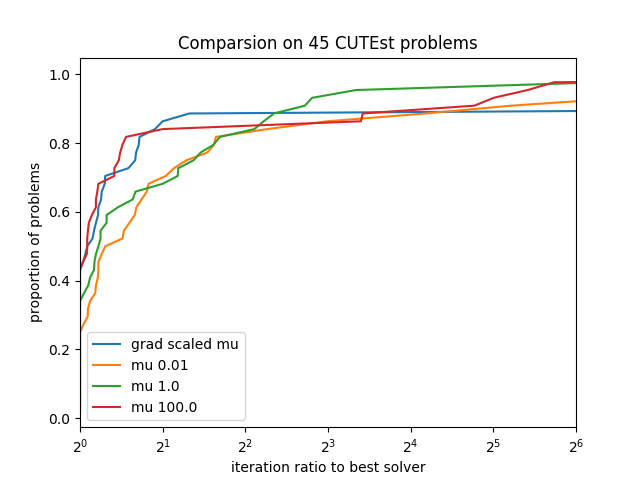
\includegraphics[scale=0.5]{mu_compare}


\end{frame}

\subsection{Netlib results} 

\startframenote
\frametitle{Duals sequence on subset of netlib}

\begin{enumerate}
\item IPOPT fails on 11/29 problems (most of these are a result of IPOPT stalling far from the optimum)
\item We fail on 4/29 (all due to numerical difficulties near the optimum).
\end{enumerate}

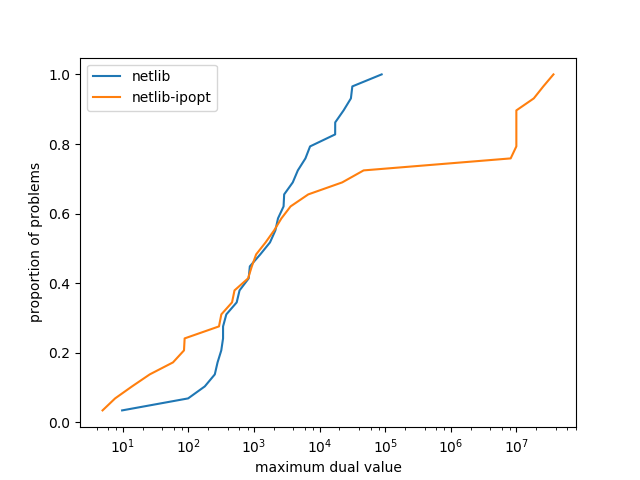
\includegraphics[scale=0.4]{duals-netlib}


\end{frame}

\subsection{CUTEst results} 

\startframenote
\frametitle{Empirical results with CUTEst}

\begin{enumerate}
\item Selected problems with $100$-$1000$ variables and $100$-$1000$ constraints.
\item Removed problems with NaNs on domain.
\end{enumerate}
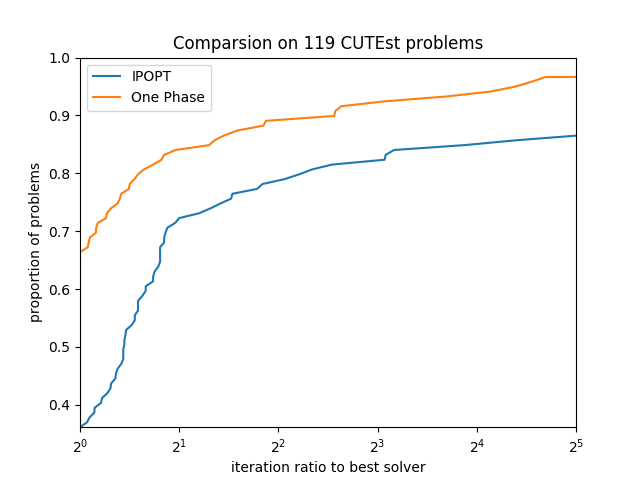
\includegraphics[scale=0.4]{cutest_vs_ipopt_correct_hess}


\end{frame}

\startframenote
\frametitle{Some infeasible problems}

\begin{center}
\begin{tabular}{ c |  c | c | }
  Problem name & IPOPT & One phase \\ 
  \hline
 MODEL & primal infeasible (29)  & primal infeasible (37) \\ 
CRESC50 & primal infeasible (491) & factorization failure (1245) \\
HIMMELBD & primal infeasible (20) & primal infeasible (35) \\
FLOSP2HL & primal infeasible (11) & primal infeasible (22) \\
FLOSP2HM & primal infeasible (16) & primal infeasible (36) \\
WOODSNE & primal infeasible (9) & primal infeasible (13) \\
ARTIF & primal infeasible (98) & optimal (15) \\
EQC & Restoration Failed! (35) & optimal (314) \\
HIMMELBJ & Restoration Failed! (28) & optimal (28) \\
%\\
%CONT6-QQ & primal infeasible (183) & primal infeasible (13) 
\end{tabular}
\end{center}

\end{frame}

\startframenote
\frametitle{Conclusions and future work}
\begin{enumerate}
\item Promising initial results
\item Look at dual values for CUTEst
\item Adaptive $\mu$ choice?
\item Better $\delta$ choice
\end{enumerate}
\end{frame}


\startframenote

\Huge{\centerline{The End}}

\end{frame}


\begin{frame}[allowframebreaks] \note{ } 

\frametitle{References}
\footnotesize{
\begin{thebibliography}{99} % Beamer does not support BibTeX so references must be inserted manually as below

\bibitem[W{\"a}chter and Biegler, 2000]{wachter2000failure} Andreas W{\"a}chter, Lorenz T. Biegler (2000)
\newblock Failure of global convergence for a class of interior point methods for nonlinear programming. \emph{Mathematical Programming}.


\bibitem[Ye et al., 1994]{hsd} Yinyu Ye, Michael J. Todd, and Shinji Mizuno (1994)
\newblock An $O (\sqrt{n}L)$-iteration homogeneous and self-dual linear programming algorithm \emph{Mathematics of Operations Research}.

\bibitem[Andersen and Ye, 1999]{homogen} Erling D. Andersen and Yinyu Ye (1999)
\newblock On a homogeneous algorithm for the monotone complementarity problem. \emph{Mathematical Programming}.

\bibitem[Lustig, 1990]{lustig1990feasibility} Irvin J Lustig (1990)
\newblock Feasibility issues in a primal-dual interior-point method for linear programming. \emph{Mathematical Programming}.

\bibitem[Mehrotra, 1992]{predictor} Mehrotra Sanjay (1992)
\newblock On the implementation of a primal-dual interior point method. \emph{SIAM Journal on optimization}.

\bibitem[Todd, 2002]{infeas-IPM} Michael J. Todd (2002)
\newblock Detecting infeasibility in infeasible-interior-point methods for optimization. \emph{Foundations of Computational Mathematics}.

\bibitem[Curtris, 2012]{curtis2012penalty} Frank E. Curtis (2012)
\newblock A penalty-interior-point algorithm for nonlinear constrained optimization. \emph{Mathematical Programming Computation}.

\bibitem[Chen, 2006]{Chen06} Lifeng Chen and Donald Goldfarb (2006)
\newblock A penalty-interior-point algorithm for nonlinear constrained optimization. \emph{Mathematical Programming}.


\end{thebibliography}
}

\end{frame}

\note{}

\end{document} 